% =====================================================================
%  Optimal blue excitation wavelength for NV-center ODMR at 120 GPa
%  Physical Review A / Applied style manuscript (REVTeX 4.2)
%
%  Compile:  pdflatex main && bibtex main && pdflatex main && pdflatex main
%
%  STATUS
%    Sec. I  (Introduction) ...... FROZEN  -- do not restructure without
%                                            re-deciding the argument chain
%                                            documented in docs/introduction_rationale.md
%    Sec. II (Model) ............. drafted from code/nv_model.py
%    Sec. III (Results Part A) ... drafted, numbers from the current code
%    Sec. IV (Results Part B) .... placeholder, awaiting PLAN.md Part B
%    Sec. V  (Calibration) ....... placeholder, awaiting PLAN.md Part C
%    Sec. VI (Conclusion) ........ drafted
% =====================================================================
\documentclass[
  aps,
  pra,
  reprint,
  amsmath,amssymb,
  floatfix,
  superscriptaddress,
  nofootinbib
]{revtex4-2}

\usepackage{graphicx}
\usepackage{bm}
\usepackage{siunitx}
\usepackage[colorlinks=true,allcolors=blue]{hyperref}

\sisetup{range-phrase=--,range-units=single}

\newcommand{\NVm}{\ensuremath{\mathrm{NV}^{-}}}
\newcommand{\NVz}{\ensuremath{\mathrm{NV}^{0}}}
\newcommand{\gsA}{\ensuremath{^{3}\!A_{2}}}
\newcommand{\esE}{\ensuremath{^{3}\!E}}
\newcommand{\sabs}{\ensuremath{\sigma_{\mathrm{abs}}}}
\newcommand{\fm}{\ensuremath{f_{-}}}
\newcommand{\lopt}{\ensuremath{\lambda_{\mathrm{opt}}}}

\begin{document}

\title{Optimal blue excitation wavelength for nitrogen-vacancy optically detected
magnetic resonance at 120~GPa}

\author{R.~Abe}
\affiliation{Institute of Science Tokyo, Tokyo, Japan}

\date{\today}

\begin{abstract}
Nitrogen-vacancy (NV) centers implanted in the culet of a diamond anvil cell have
become the reference local probe of magnetism in the megabar regime, where they
provide the diamagnetic and flux-trapping signatures that establish
superconductivity in hydrogen-rich compounds. Their usefulness there is limited
not by whether optically detected magnetic resonance (ODMR) survives compression,
but by how fast a given magnetic sensitivity can be reached. We show that at
\SI{120}{\giga\pascal} this sensitivity is controlled almost entirely by a single
experimental choice that is usually inherited from ambient-pressure practice: the
excitation wavelength. Using a rate-equation model of the lock-in ODMR
sensitivity $\eta \propto \Delta\nu/(C\sqrt{R})$ whose optical and charge-transfer
inputs are anchored to first-principles and experimental photophysics of the NV
center up to \SI{120}{\giga\pascal}, we find that the pressure-induced blue shift
of the zero-phonon line and the strengthening of the electron-phonon coupling
displace the optimal excitation into a narrow window centered at
$\lambda_{\mathrm{opt}} = \SI{475}{\nano\meter}$, while the concurrent rise of
the ground-state photoionization threshold to
$\mathrm{IP}(^{3}\!A_{2}) = \SI{3.06}{\electronvolt}$ imposes a hard blue
boundary at \SI{405}{\nano\meter}. Both conventional choices fall outside the
window, for different reasons: \SI{532}{\nano\meter} is degraded by a factor
$5.2$ because the absorption onset has moved past it, and \SI{405}{\nano\meter}
by a factor $4.2$ because it sits on the far blue flank of the absorption
envelope, with direct ground-state ionization switching on immediately beyond
it. Inside the window the steady-state charge state is nearly wavelength
independent---excited-state ionization and recombination both scale with the
absorption cross section and largely cancel from the \NVm{} fraction---so the
fixed-power optimum coincides with the maximum of the Franck-Condon absorption
envelope, a specific prediction that the proposed two-beam calibration is
designed to test. The $5\%$ tolerance window,
\SIrange{463}{486}{\nano\meter}, contains the commercial \SI{473}{\nano\meter}
line, which is therefore predicted to be operationally optimal.
\end{abstract}

\maketitle

% =====================================================================
\section{Introduction}
% ---------------------------------------------------------------------
% FROZEN. Argument chain (see docs/introduction_rationale.md):
%   (i)   hydride superconductivity needs LOCAL magnetic evidence
%   (ii)  NV-in-anvil is the only probe that delivers it
%   (iii) the relevant pressures cluster around 100-140 GPa
%   (iv)  the bottleneck is ODMR SENSITIVITY, not survival
%   (v)   at 120 GPa three photophysical shifts break ambient-pressure
%         excitation practice, and they pull in opposite directions
%   (vi)  nobody has computed where the resulting optimum actually is
%   (vii) this work
% ---------------------------------------------------------------------
\label{sec:intro}

The search for superconductivity in hydrogen-rich compounds, initiated by
Ashcroft's proposal that metallic hydrogen and hydrogen-dominant alloys should be
high-temperature superconductors~\cite{Ashcroft1968,Ashcroft2004}, has produced
the highest critical temperatures on record: \SI{203}{\kelvin} in
H$_3$S at \SI{155}{\giga\pascal}~\cite{Drozdov2015} and \SIrange{250}{260}{\kelvin}
in LaH$_{10}$ near \SI{170}{\giga\pascal}~\cite{Drozdov2019,Somayazulu2019}. A
second family of clathrate superhydrides operates at markedly lower
pressure: CeH$_9$ is synthesized at \SIrange{80}{100}{\giga\pascal} and
superconducts with $T_c$ up to \SI{115}{\kelvin} below one
megabar~\cite{Salke2019,Chen2021CeH9}, and the substitutional alloy
(La,Ce)H$_9$ reaches \SIrange{148}{178}{\kelvin} over
\SIrange{97}{172}{\giga\pascal}~\cite{Semenok2022LaCeH9}. These materials are the
most attractive near-term targets precisely because their working pressures,
clustered around \SI{120}{\giga\pascal}, are compatible with a well-characterized
diamond anvil cell (DAC) rather than with an extreme, low-yield one.

What has not kept pace is the \emph{evidence}. A sample in a DAC at
\SI{120}{\giga\pascal} occupies a culet of a few tens of micrometers and a volume
of order picoliters, so conventional bulk magnetometry cannot isolate its
diamagnetic response from the anvil and gasket background~\cite{Minkov2022}.
Resistive signatures alone have repeatedly proved insufficient to settle claims of
superconductivity in this field, which has made a direct, local, and spatially
resolved measurement of magnetic flux expulsion the decisive experiment rather
than a confirmatory one.

NV centers implanted a few tens of nanometers beneath the culet surface supply
exactly this measurement. Because the sensor layer is fabricated \emph{inside}
the anvil, it sits micrometers from the sample and survives the same pressure the
sample does; ODMR then reports the local magnetic field and the local stress
tensor simultaneously~\cite{Doherty2014,Hsieh2019,Lesik2019,Yip2019}. This
capability has been pushed from the \SI{30}{\giga\pascal} scale to
\SI{130}{\giga\pascal}~\cite{Hilberer2023}, to megabar
pressures~\cite{Dai2022,Wang2024}, and most recently to
\SI{240}{\giga\pascal}~\cite{Hao2025}. Its highest-profile application to date is
the imaging of the Meissner effect and of flux trapping in CeH$_9$ at megabar
pressures, which resolved the superconducting regions and showed that they are
strongly inhomogeneous on the micron scale~\cite{Bhattacharyya2024}; comparable
measurements have since been reported for LaH$_{10}$~\cite{ChenLaH2025}, for
conventional superconductors under pressure~\cite{Dailledouze2025}, and for
pressurized nickelates~\cite{Mandyam2026}.

That last result identifies the bottleneck. The scientific content of these
experiments is carried by \emph{maps}---the spatial texture of the screening
field, the geometry of trapped flux---and by their evolution through $T_c$ and
with pressure. A map is a raster of ODMR spectra, so the total measurement time
scales as the number of pixels divided by the square of the magnetic sensitivity
$\eta_B$~\cite{Barry2020}. In a regime where a single successful loading takes
weeks to prepare and can be lost in one anvil failure, sensitivity is not a
figure of merit but the currency in which spatial resolution, field-of-view, and
the number of accessible $(P,T)$ points are all purchased. The relevant question
for NV sensing at \SI{120}{\giga\pascal} is therefore not whether ODMR survives
compression---recent photophysical work shows convincingly that it
does~\cite{Ho2026,Huang2025ISC}---but how to make it as sensitive as possible
there.

The answer is constrained by the fact that the NV center at
\SI{120}{\giga\pascal} is optically a different emitter from the one at ambient
pressure, in three ways that a recent combined \emph{ab initio} and experimental
study has now quantified~\cite{Ho2026}. First, the \NVm{} zero-phonon line (ZPL)
blue-shifts by more than \SI{0.4}{\electronvolt}, from \SI{1.945}{\electronvolt}
to $\simeq\SI{2.35}{\electronvolt}$ (\SI{529}{\nano\meter}). The
\SI{532}{\nano\meter} line, which at ambient pressure excites comfortably into the
phonon sideband, therefore lands \emph{at} the absorption onset at
\SI{120}{\giga\pascal}, where the cross section has collapsed. Excitation must
move into the blue; this is a constraint, not a preference. Second, the
electron-phonon coupling strengthens substantially---the absorption Huang-Rhys
factor of the Jahn-Teller-inactive modes rises from $3.08$ to $4.61$ and the
absorption Debye-Waller factor falls from $2.2\%$ to $0.36\%$---so the absorption
envelope both broadens and moves its weight to higher energy, placing its
maximum near \SI{475}{\nano\meter}. Third, the photoionization thresholds shift
upward as well: $\mathrm{IP}(\gsA)$ rises from \SI{2.68}{\electronvolt} to
\SI{3.06}{\electronvolt} and $\mathrm{IP}(\esE)$ from \SI{1.16}{\electronvolt} to
\SI{1.63}{\electronvolt}~\cite{Ho2026,Razinkovas2021}. Since
\SI{3.06}{\electronvolt} corresponds to \SI{405}{\nano\meter}, the
\SI{405}{\nano\meter} diode line that is standard for charge-state manipulation
sits exactly on the ground-state ionization edge at \SI{120}{\giga\pascal}: it is
the last wavelength before one-photon ionization out of \gsA{} switches on, and
everything bluer converts \NVm{} directly into \NVz{}.

The three shifts do not act in the same direction, and that is what makes the
problem nontrivial. Moving the excitation bluer follows the displaced absorption
band and buys photon rate; moving it bluer also approaches the ground-state
ionization edge, depletes the steady-state \NVm{} fraction $\fm$, and dilutes the
ODMR contrast with unpolarized \NVz{} fluorescence. The lock-in sensitivity,
$\eta \propto \Delta\nu/(C\sqrt{R})$, weighs these against each other with
different powers---linearly in contrast, as a square root in photon rate---so
where the balance falls is a quantitative question and not one that can be
settled by inspecting the absorption spectrum. Reference~\cite{Ho2026} recognizes
the issue and states the
qualitative guideline that the excitation should be tuned to follow the ZPL
shift, but stops short of the quantitative question that an experimenter has to
answer when specifying a laser: \emph{which} wavelength, to what tolerance, and
whether that choice depends on the optical power---a question with direct
consequences in a DAC, where the culet is small, the sample is metallic and
absorbing, and the usable power is capped by heating rather than by the laser.

Here we answer that question. We construct a rate-equation model of the CW lock-in
ODMR sensitivity in which the absorption cross section, the ionization thresholds,
and the electron-phonon parameters are taken from the \SI{120}{\giga\pascal}
photophysics of Ref.~\cite{Ho2026}, and only the charge-transfer rate constants
and the \NVz{} background weight remain phenomenological. Minimizing $\eta$ over
the blue excitation window at \SI{120}{\giga\pascal} yields an optimum at
$\lopt = \SI{475}{\nano\meter}$. The balance turns out to be resolved in a
specific and testable way: within the blue window the two intensity-linear charge
channels---excited-state ionization and recombination---both scale with $\sabs$
and cancel from $\fm$ to better than $0.2\%$, so at fixed power the optimum is
fixed by the photon rate and coincides with the maximum of the absorption
envelope, while the ionization physics enters as a hard boundary at
\SI{405}{\nano\meter} rather than as a detuning of the optimum. Relative to the
optimum, \SI{532}{\nano\meter} costs a factor $5.2$ and \SI{405}{\nano\meter} a
factor $4.2$ in sensitivity, while the $5\%$ tolerance window
\SIrange{463}{486}{\nano\meter} contains the commercial \SI{473}{\nano\meter}
line at a cost of $0.1\%$. We further show that $\lopt$ tracks the ZPL at
\SIrange{0.6}{0.7}{\nano\meter\per\giga\pascal}, so that the choice must be made
per target pressure, and we identify which of the underlying photophysical
anchors the answer is most sensitive to, and hence which quantities a calibration
experiment should pin down first.

% =====================================================================
\section{Model}
\label{sec:model}

\subsection{Sensitivity functional}

For continuous-wave, lock-in-detected ODMR the shot-noise-limited magnetic
sensitivity is~\cite{Barry2020,Dreau2011,Rondin2014}
\begin{equation}
  \eta_B \;\simeq\; \mathcal{P}\,\frac{h}{g\mu_B}\,
  \frac{\Delta\nu}{C\sqrt{R}} ,
  \label{eq:eta}
\end{equation}
with $\Delta\nu$ the ODMR linewidth, $C$ the resonance contrast, $R$ the detected
photon rate, and $\mathcal{P}$ a lineshape factor of order unity. Since the
excitation wavelength enters only through $\Delta\nu$, $C$ and $R$, we work
throughout with the reduced quantity $\eta \equiv \Delta\nu/(C\sqrt{R})$ in
arbitrary units, and quote all results as ratios $\eta(\lambda)/\eta(\lopt)$,
which are independent of the overall scale.

\subsection{Pressure-dependent optical inputs}

All optical quantities are anchored to Ref.~\cite{Ho2026}. The ZPL energy is
represented by a saturating form
\begin{equation}
  E_{\mathrm{ZPL}}(P) = \SI{1.945}{\electronvolt}
  + E_{\max}\left[1 - e^{-P/P_0}\right],
\end{equation}
with $E_{\max} = \SI{0.758}{\electronvolt}$ and $P_0 = \SI{160}{\giga\pascal}$,
reproducing the reported shift of $>\SI{0.4}{\electronvolt}$ at
\SI{120}{\giga\pascal}. The absorption Huang-Rhys factor of the
Jahn-Teller-inactive modes and the two photoionization thresholds are taken
linear in $P$ between their reported end points,
\begin{align}
  S_{\mathrm{abs}}(P) &= 3.08 + (4.61-3.08)\,P/P_{120},\\
  \mathrm{IP}(\gsA)(P) &= \SI{2.68}{\electronvolt}
    + \SI{0.38}{\electronvolt}\,P/P_{120},\\
  \mathrm{IP}(\esE)(P) &= \SI{1.16}{\electronvolt}
    + \SI{0.47}{\electronvolt}\,P/P_{120},
\end{align}
with $P_{120} \equiv \SI{120}{\giga\pascal}$. The absorption cross section is a
low-temperature Franck-Condon (Pekarian) envelope built on an effective phonon
energy $\hbar\omega = \SI{65}{\milli\electronvolt}$~\cite{Kehayias2013,Huang1950},
\begin{equation}
  \sabs(E,P) \;\propto\;
  e^{-S_{\mathrm{abs}}}\,\frac{S_{\mathrm{abs}}^{\,n}}{n!}
  \Big|_{\,n = (E-E_{\mathrm{ZPL}})/\hbar\omega}
  \;+\; \mathrm{DWF}(P)\,\delta_{\mathrm{ZPL}}(E),
  \label{eq:sigma}
\end{equation}
normalized so that $\sabs(\SI{532}{\nano\meter}, 0) = 1$, with the narrow ZPL
component weighted by the reported absorption Debye-Waller factor falling from
$2.2\%$ to $0.36\%$.

\subsection{Charge state and contrast}

The steady-state \NVm{} fraction follows from the balance of photoionization and
recombination,
\begin{equation}
  \fm = \frac{G_{\mathrm{rec}}}{G_{\mathrm{rec}} + G_{\mathrm{ion}}},
\end{equation}
with the two ionization channels identified in
Refs.~\cite{Aslam2013,Razinkovas2021,Ho2026},
\begin{align}
  G_{\mathrm{ion}} &= a_{\mathrm{gs}}\,
      \big[E_\gamma - \mathrm{IP}(\gsA)\big]_{+}
    \;+\; a_{\mathrm{es}}\,\sabs ,
  \label{eq:gion}\\
  G_{\mathrm{rec}} &= r_0\,\sabs + r_{\mathrm{bg}} ,
\end{align}
where $[\,\cdot\,]_{+}$ denotes the positive part: the first term is one-photon
ionization directly out of \gsA{}, which switches on abruptly above the
ground-state threshold, and the second is the two-step process proceeding via
\esE{}. Fluorescence from \NVz{} is unpolarized and therefore dilutes the ODMR
contrast,
\begin{equation}
  C = C_0\,\frac{\fm}{\fm + w_0\,(1-\fm)},
\end{equation}
with $w_0$ the relative brightness of the \NVz{} background, while the detected
rate is $R \propto \fm\,\sabs$ at fixed excitation power. The linewidth
$\Delta\nu(P)$ carries only a mild strain-broadening term and is independent of
$\lambda$, so it does not affect $\lopt$ at fixed power.

The rate constants $\{a_{\mathrm{gs}}, a_{\mathrm{es}}, r_0, r_{\mathrm{bg}},
w_0\}$ are phenomenological; they are the targets of the calibration described in
Sec.~\ref{sec:calibration}, and their influence on the results is propagated
throughout by Monte Carlo.

% =====================================================================
\section{Optimal blue wavelength at 120~GPa}
\label{sec:resultsA}

\begin{figure}[t]
  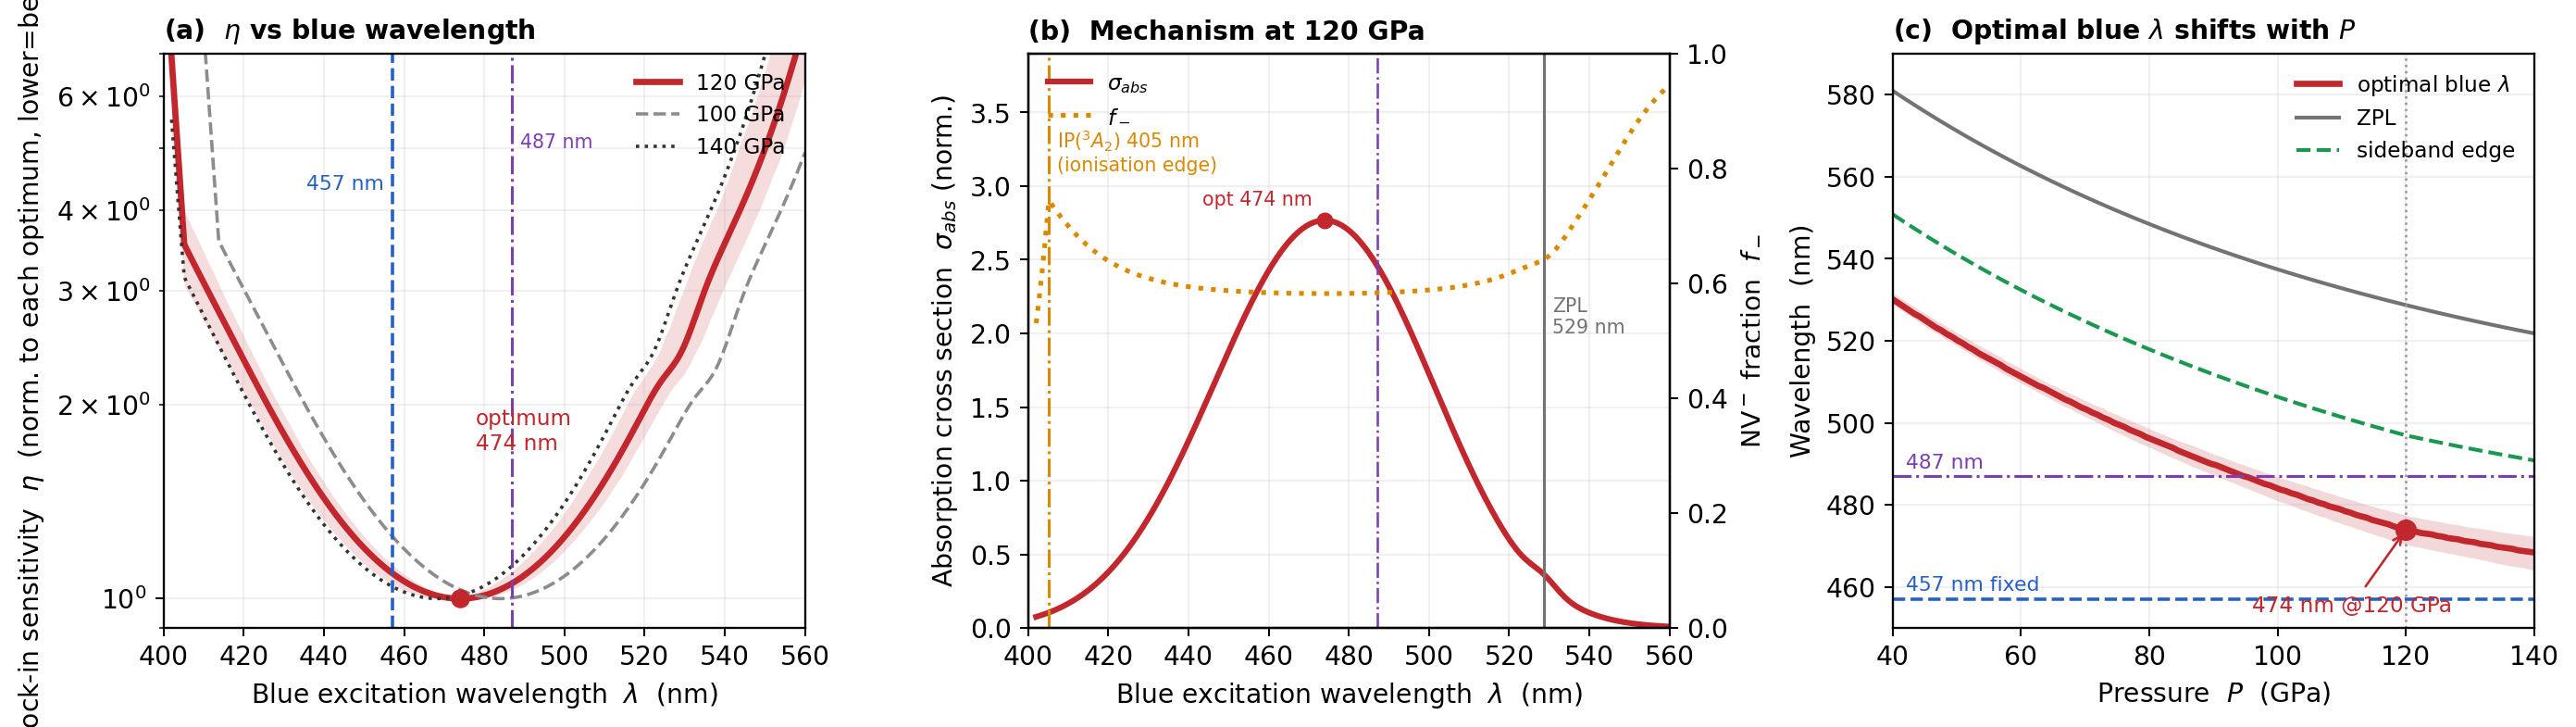
\includegraphics[width=\linewidth]{../code/blue_wavelength_sensitivity_120GPa.png}
  \caption{(a) Reduced lock-in sensitivity $\eta(\lambda)$ at
  \SI{120}{\giga\pascal} (normalized to its own optimum) with the Monte Carlo
  $16$--$84\%$ band, compared with \SI{100}{\giga\pascal} and
  \SI{140}{\giga\pascal}. (b) Mechanism: the absorption cross section $\sabs$ and
  the steady-state \NVm{} fraction $\fm$, with the ZPL and the ground-state
  ionization edge marked. (c) The optimal blue wavelength as a function of
  pressure, tracking the ZPL and the sideband edge.}
  \label{fig:sweep}
\end{figure}

At \SI{120}{\giga\pascal} the model inputs give
$E_{\mathrm{ZPL}} = \SI{2.345}{\electronvolt}$ (\SI{529}{\nano\meter}),
$S_{\mathrm{abs}} = 4.61$, and $\mathrm{IP}(\gsA) = \SI{3.06}{\electronvolt}$
(\SI{405.2}{\nano\meter}). The Franck-Condon envelope of Eq.~\eqref{eq:sigma}
then peaks at \SI{474.8}{\nano\meter}; note that this is not the discrete
Poisson mean $E_{\mathrm{ZPL}} + S_{\mathrm{abs}}\hbar\omega$, which would place
the maximum at \SI{469}{\nano\meter}, because the continuous vibronic envelope is
skewed relative to its phonon-number mean. Minimizing Eq.~\eqref{eq:eta} over
$\lambda$ yields
\begin{equation}
  \lopt(\SI{120}{\giga\pascal}) = \SI{474.8}{\nano\meter},
\end{equation}
coincident with the absorption maximum to the resolution of the grid.

That coincidence is a result, not a triviality, and it identifies which physics
actually sets the answer. Over the whole blue window the steady-state charge
state is essentially flat: $\fm$ varies from $0.5806$ to $0.5816$ across
\SIrange{463}{486}{\nano\meter} [Fig.~\ref{fig:sweep}(b)]. The reason is
structural. Above the ionization edge the ReLU term of Eq.~\eqref{eq:gion}
vanishes, so both surviving channels---excited-state ionization $a_{\mathrm{es}}
\sabs$ and recombination $r_0 \sabs$---are proportional to the same cross
section, and $\sabs$ cancels from $\fm$ except through the constant dark term
$r_{\mathrm{bg}}$. At fixed excitation power the wavelength dependence of $\eta$
is therefore carried almost entirely by $R \propto \sabs$, and the optimum is the
absorption maximum. Setting $a_{\mathrm{gs}} = 0$ leaves $\lopt$ unchanged to
within the grid spacing, confirming that ground-state ionization does not
displace the optimum; it acts instead as a boundary that forbids the region blueward of
\SI{405}{\nano\meter}. This is a falsifiable prediction of the model rather than
a generic expectation: it holds only as long as the excited-state ionization and
recombination channels share the same spectral dependence, which is exactly what
the two-beam calibration of Sec.~\ref{sec:calibration} is designed to test, and
which the power-explicit treatment of Sec.~\ref{sec:resultsB} relaxes.

Table~\ref{tab:lines} lists the penalty incurred by the commercially available
laser lines. Two entries carry the practical message, and they fail for opposite
reasons. The \SI{532}{\nano\meter} line, still the default in most NV setups, is
degraded by a factor $5.2$ because at this pressure it excites
\SI{3}{\nano\meter} to the red of the ZPL, where $\sabs$ has fallen to $4\%$ of
its ambient-pressure green value---a factor of $83$ below $\sabs$ at
\SI{475}{\nano\meter}. The \SI{405}{\nano\meter} line is degraded by a comparable
factor $4.2$ because it lies far out on the blue flank of the envelope, where
$\sabs = 0.085$; the ground-state ionization term contributes only $9\%$ of the
total ionization rate there, since \SI{405}{\nano\meter} sits barely above
threshold. Its significance is that there is no room to move further blue: the
ReLU term grows linearly with detuning above $\mathrm{IP}(\gsA)$, so the
\SI{405}{\nano\meter} line marks the edge of the usable spectrum rather than a
usable operating point.

\begin{table}[t]
  \caption{Sensitivity penalty $\eta(\lambda)/\eta(\lopt)$ of commercial laser
  lines at \SI{120}{\giga\pascal} (lower is better; $1.000$ is optimal).}
  \label{tab:lines}
  \begin{ruledtabular}
  \begin{tabular}{lcl}
    $\lambda$ (nm) & $\eta/\eta_{\mathrm{opt}}$ & comment \\ \colrule
    405 & 4.23  & blue flank; at the $\mathrm{IP}(\gsA)$ edge \\
    457 & 1.12  & inside the $10\%$ window \\
    473 & 1.00  & \textbf{operationally optimal} \\
    475 & 1.00  & model optimum \\
    488 & 1.07  & inside the $10\%$ window \\
    505 & 1.44  & outside \\
    532 & 5.16  & at the absorption onset \\
  \end{tabular}
  \end{ruledtabular}
\end{table}

The tolerance windows are \SIrange{463}{486}{\nano\meter} at the $5\%$ level and
\SIrange{458}{491}{\nano\meter} at the $10\%$ level. The commercial
\SI{473}{\nano\meter} DPSS line lies \SI{2}{\nano\meter} from the optimum and
costs $0.1\%$; it is therefore the recommended practical choice, and no custom
source is required.

Finally, $\lopt$ is not a constant of the technique but of the pressure:
Fig.~\ref{fig:sweep}(c) shows that it tracks the ZPL and the sideband edge at
\SIrange{0.6}{0.7}{\nano\meter\per\giga\pascal}, moving from
\SI{487}{\nano\meter} at \SI{100}{\giga\pascal} to \SI{475}{\nano\meter} at
\SI{120}{\giga\pascal}. Over the \SIrange{97}{172}{\giga\pascal} window spanned
by the (La,Ce)H$_9$ family~\cite{Semenok2022LaCeH9} this amounts to a shift
larger than the $10\%$ tolerance band, so the excitation wavelength has to be
selected for the target pressure rather than for the technique.

% =====================================================================
\section{Power dependence of the optimum}
\label{sec:resultsB}

% PLACEHOLDER -- PLAN.md Part B.
% Model extension: two-photon ionisation via 3E (quadratic at low u, saturating
% at high u), saturation of the excited-state population and of R, and the
% standard CW-ODMR power broadening of C and of the linewidth.
% Deliverable: eta(lambda,u) map at 120 GPa, the ridge lambda_opt(u) with its
% Monte-Carlo band, and the contribution decomposition (two-photon ionisation /
% R saturation / power broadening) that explains the direction of the shift.

\emph{[To be completed from the power-explicit model
(\texttt{code/nv\_model\_power.py}); see Part~B of the project plan.]}

% =====================================================================
\section{Calibration of the phenomenological rates}
\label{sec:calibration}

% PLACEHOLDER -- PLAN.md Part C.
% Two-beam (405 nm, 457 nm) intensity sweep; least-squares + MCMC fit of
% {a_gs, a_es', r0, r_bg, Gamma_sat, w0}; identifiability check by profile
% likelihood before the measurement is run; posterior propagated into the
% lambda_opt(u) band.

\emph{[To be completed; see Part~C of the project plan.]}

% =====================================================================
\section{Conclusion}
\label{sec:conclusion}

The pressure-induced reorganization of NV photophysics at
\SI{120}{\giga\pascal}---a ZPL blue shift beyond \SI{0.4}{\electronvolt}, a
$50\%$ increase of the absorption Huang-Rhys factor, and a concurrent rise of the
ground-state photoionization threshold to \SI{3.06}{\electronvolt}---places the
optimal ODMR excitation in a narrow blue window centered at
\SI{475}{\nano\meter}. Both conventional choices lie far outside it, and for
opposite physical reasons: \SI{532}{\nano\meter} because absorption has collapsed
at the shifted onset, \SI{405}{\nano\meter} because it lies on the far blue flank
of the envelope with the ionization edge immediately beyond. Within the window
the charge state is nearly wavelength independent, since the excited-state
ionization and recombination channels share the same $\sabs$ dependence and
cancel from $\fm$; at fixed power the optimum is therefore the absorption maximum
itself, and it tracks the ZPL at
\SIrange{0.6}{0.7}{\nano\meter\per\giga\pascal}. Whether that cancellation
survives---at high intensity, where excited-state ionization becomes a two-photon
process and recombination proceeds through the separate \NVz{} absorption
envelope, it should not---is the question the power-explicit treatment and the
two-beam calibration are designed to settle. The practical consequence is
immediate: a \SI{473}{\nano\meter} source recovers essentially the full optimum
at \SI{120}{\giga\pascal}, and buys back a factor of $\simeq 5$ in sensitivity
relative to green excitation---equivalently a factor of $\simeq 25$ in the
acquisition time of a magnetic map, in a class of experiment where measurement
time is the binding constraint.

\begin{acknowledgments}
\emph{[To be completed.]}
\end{acknowledgments}

\bibliographystyle{apsrev4-2}
\bibliography{refs}

\end{document}
